% \begin{table}
%     \caption{Mô hình học tăng cường khác môi trường}
%     \begin{center}
%     \begin{tabular}{|c|c|c|c|c|c|}
%     \hline
%     \multirow{1}{*}{\textbf{Trọng lực}} &
%     \multirow{1}{*}{\textbf{Method}} & \multicolumn{1}{c|}{\textbf{Cao nhất}} & {\textbf{Thấp nhất}} & \multicolumn{1}{c|}{\textbf{Trung Bình}} & \multicolumn{1}{c|}{\textbf{Độ lệch}} \\ \hline
%     \multirow{3}{*} 
%     {Trọng lực=1.0} &
%     CEA & $71$ & $4$ & $28.86$ & $17.16$ \\
%     & MFEAI & $\mathbf{129}$ & $17$ &$46.71$ & $20.36$  \\
%     & MFEAII & $84$ & $15$ & $\mathbf{52.81}$  &$15.45$\\\hline
%     \multirow{3}{*} 
%     {Trọng lực=1.98} &
%     CEA & $382$ & $7$ &$174.86$ & $113.79$ \\
%     & MFEAI  & $\mathbf{546}$ & $98$ & $\mathbf{319.86}$ & $95.34$ \\
%     & MFEAII & $517$ & $\mathbf{131}$ &$311.38$ & $106.76$ \\\hline
%     \multirow{3}{*} 
%     {Trọng lực=2.96} &
%     CEA & $272$ & $1$ &$97.9$ & $83.07$ \\
%     & MFEAI  & $\mathbf{349}$ & $\mathbf{140}$ & $\mathbf{222.81}$ & $52.07$ \\
%     & MFEAII & $322$ & $103$ &$212.38$ & $52.74$ \\\hline
%     \multirow{3}{*} 
%     {Trọng lực=3.94} &
%     CEA & $227$ & $2$ &$69.24$ & $56.64$ \\
%     & MFEAI  & $\mathbf{217}$ & $\mathbf{95}$ & $\mathbf{142.86}$ & $27.4$ \\
%     & MFEAII & $190$ & $76$ &$140.38$ & $27.78$ \\\hline
%     \multirow{3}{*} 
%     {Trọng lực=4.92} &
%     CEA & $95$ & $2$ & $25.48$ & $25.78$  \\
%     & MFEAI  & $\mathbf{181}$ & $\mathbf{54}$ & $90.86$ & $21.98$ \\
%     & MFEAII & $145$ & $44$ & $\mathbf{102.14}$ & $26.66$ \\\hline
%     \end{tabular}
%     \end{center}
    
%     \label{tab:result:nbit}
% \end{table}

\subsubsection{Bảng kết quả thực nghiệm - bài toán Acrobot}
\begin{table} [H]
    \begin{center}
    \caption{Kết quả huấn luyện các tác vụ cho bài toán Acrobot}

    \scalebox{0.9}{\begin{tabular}{|c|c|c|c|c|c|}
    \hline
    \multirow{1}{*}{\textbf{Thuật toán}} & \multicolumn{1}{c|}{\textbf{Tác vụ 1}} & \multicolumn{1}{c|}{\textbf{Tác vụ 2}} & \multicolumn{1}{c|}{\textbf{Tác vụ 3}} & \multicolumn{1}{c|}{\textbf{Tác vụ 4}} & \multicolumn{1}{c|}{\textbf{Tác vụ 5}} \\ \hline
    CEA & $-100 \pm 4.53$ & $-109.47 \pm 2.38$ & $-108.77 \pm 4.38$ & $-113.17 \pm 1.86$ & $-117.23 \pm 4.28$  \\
    MFEAI &  $-100 \pm 4.75$ & $\mathbf{-106.7 \pm 0.78}$ & $\mathbf{-108.3 \pm 4.47}$ & $-112.0 \pm 2.62$ & $-117.03 \pm 4.52$ \\
    MFEAII & $\mathbf{-100 \pm 4.7}$ & $-107.8 \pm 1.17$ & $-108.6 \pm 4.34$ & $\mathbf{-113.07 \pm 2.29}$ & $\mathbf{-116.9 \pm 4.09}$  \\\hline
    \end{tabular}}
    \end{center}
    \label{tab:result:acrobot}
\end{table}


\subsubsection{Biểu đồ hội tụ - bài toán Acrobot}
\begin{figure}[h!]
    \centering
    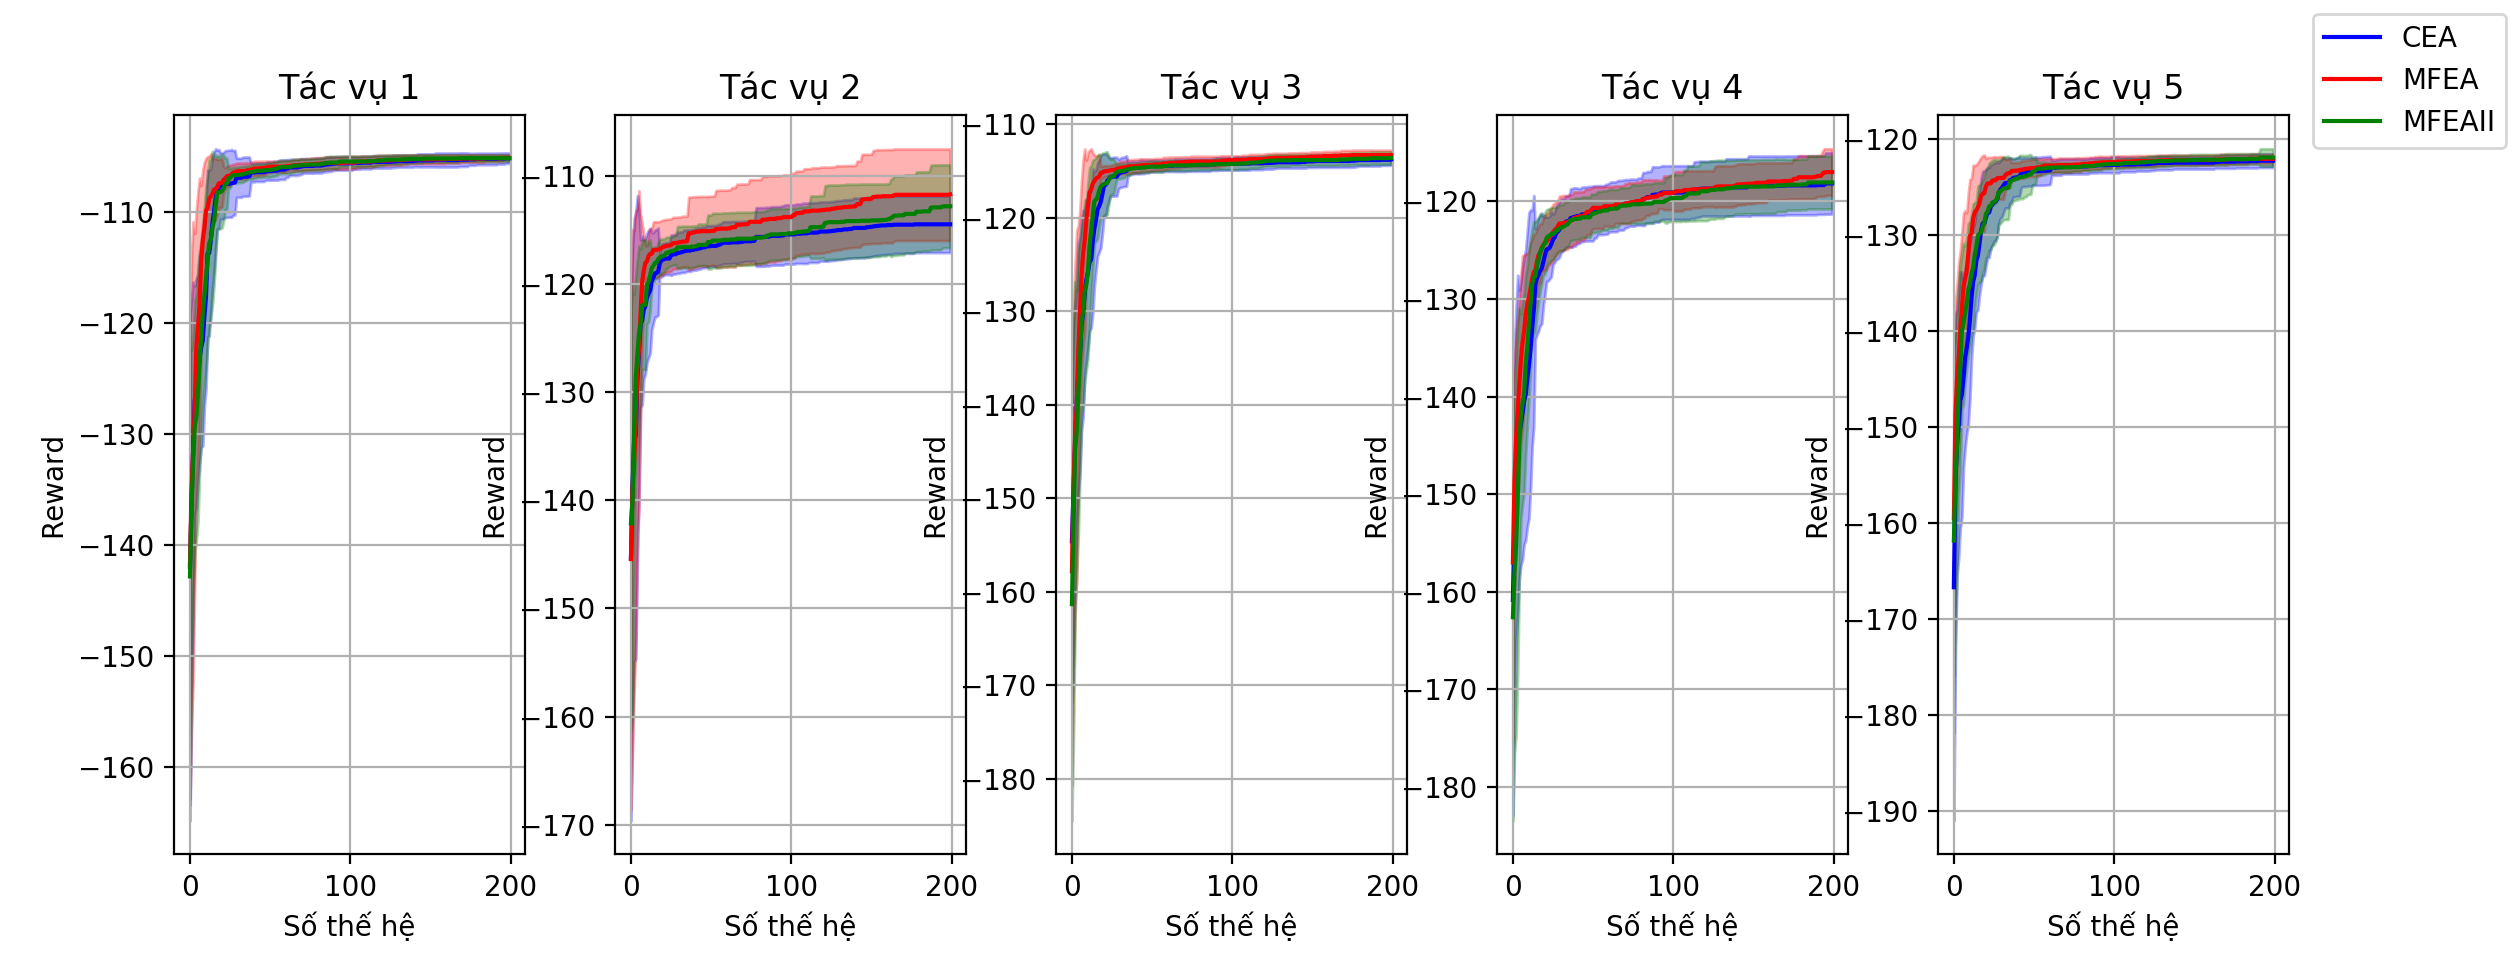
\includegraphics[width=\textwidth,height=\textheight,keepaspectratio]{thesis/images/results/rl/acrobot_conv.png}
    \caption{Biểu đồ hội tụ các tác vụ cho bài toán Acrobot}
    \label{fig:Acrobot_conv}
\end{figure}

\subsubsection{So sánh mức độ tập trung kết quả cuối cùng - bài toán Acrobot}
\begin{figure}[h!]
    \centering
    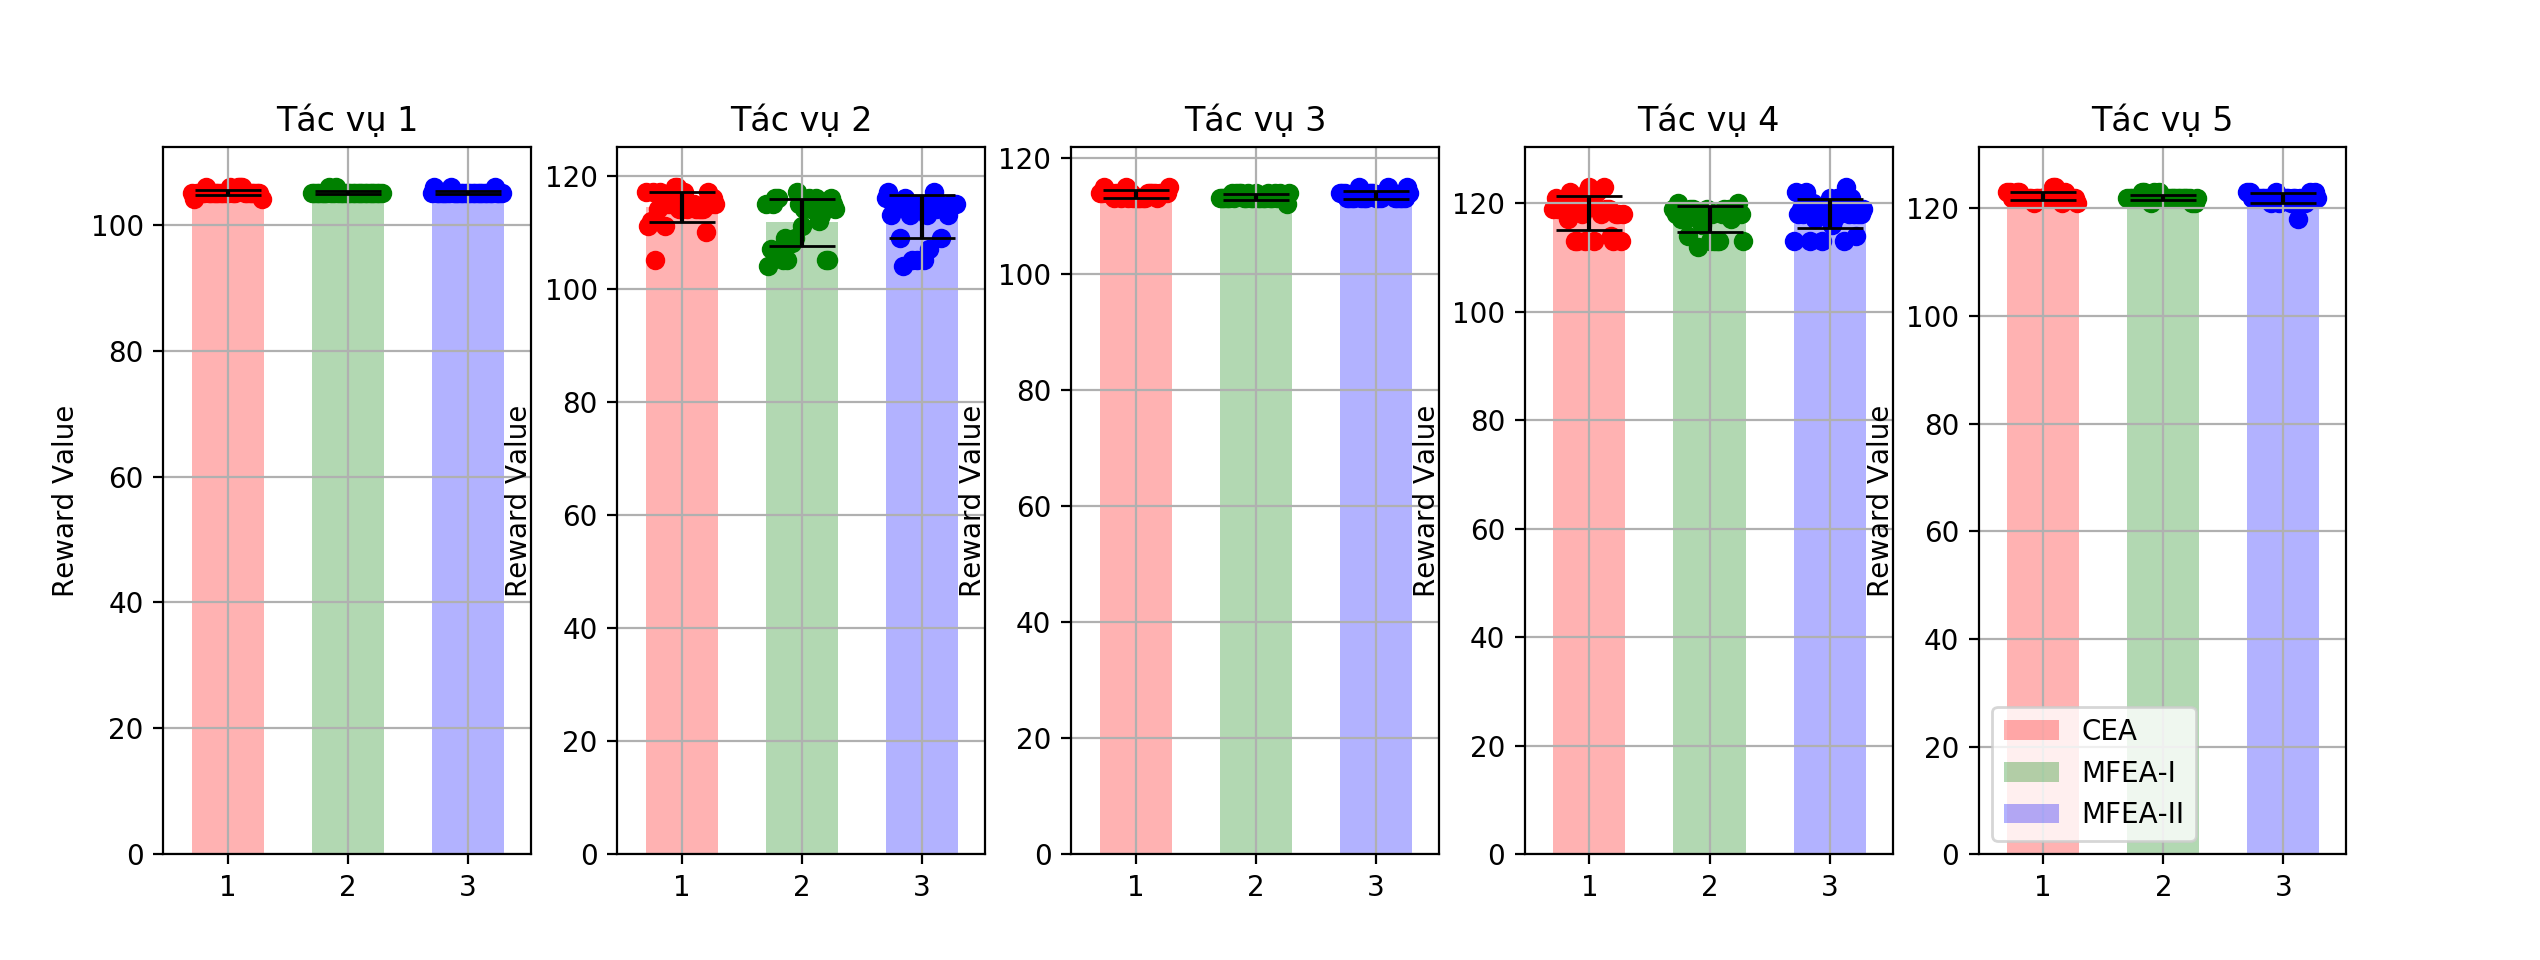
\includegraphics[width=\textwidth,height=\textheight,keepaspectratio]{thesis/images/results/rl/acrobot_final.png}
    \caption{Biểu đồ so sánh mức độ tập trung kết quả cuối cùng cho bài toán Acrobot (khi so sánh trị tuyệt đối của kết quả)}
    \label{fig:Acrobot}
\end{figure}


\subsubsection{Bảng kết quả thực nghiệm - bài toán PixelCopter}
\begin{table} [h!]
    \begin{center}
    \caption{Kết quả huấn luyện các tác vụ cho bài toán PixelCopter}

    \scalebox{0.9}{\begin{tabular}{|c|c|c|c|c|c|}
    \hline
    \multirow{1}{*}{\textbf{Thuật toán}} & \multicolumn{1}{c|}{\textbf{Tác vụ 1}} & \multicolumn{1}{c|}{\textbf{Tác vụ 2}} & \multicolumn{1}{c|}{\textbf{Tác vụ 3}} & \multicolumn{1}{c|}{\textbf{Tác vụ 4}} & \multicolumn{1}{c|}{\textbf{Tác vụ 5}} \\ \hline
    CEA & $101.97 \pm 26.15$ & $104.6 \pm 23.16$ & $96.83 \pm 22.74$ & $96.67 \pm 28.27$ & $93.47 \pm 19.09$ \\
    MFEAI & $124.47 \pm 32.08$ & $125.93 \pm 31.4$ & $123.43 \pm 24.86$ & $122.33 \pm 23.08$ & $120.37 \pm 30.36$  \\
    MFEAII & $\mathbf{133.57 \pm 28.29}$ & $\mathbf{132.03 \pm 33.31}$ & $\mathbf{132.73 \pm 26.93}$ & $\mathbf{129.0 \pm 22.93}$ & $\mathbf{135.4 \pm 30.11}$ \\\hline
    \end{tabular}}
    \end{center}
    \label{tab:result:pixelcopter}
\end{table}


\subsubsection{Biểu đồ hội tụ - bài toán PixelCopter}
\begin{figure}[h!]
    \centering
    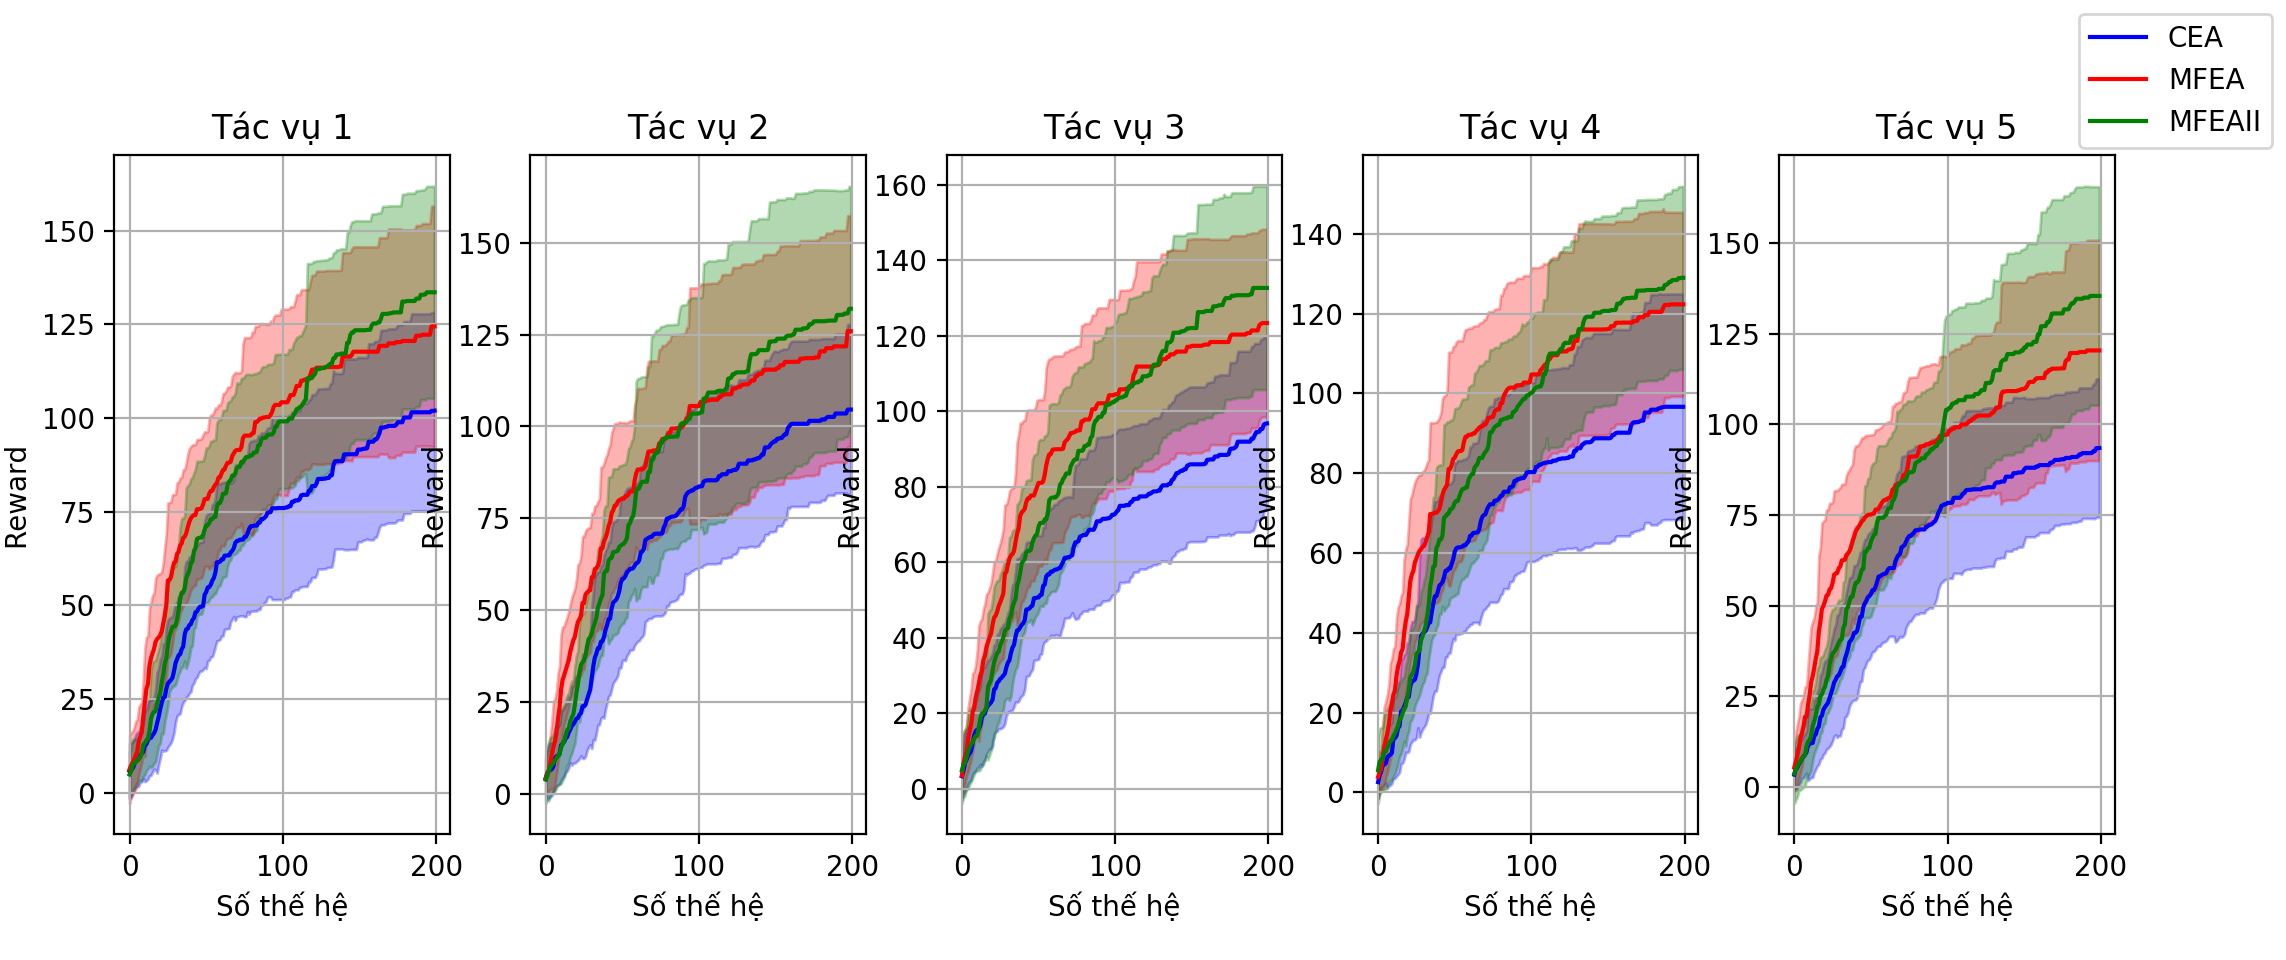
\includegraphics[width=\textwidth,height=\textheight,keepaspectratio]{thesis/images/results/rl/pixcelcopter_conv.png}
    \caption{Biểu đồ hội tụ các tác vụ cho bài toán PixelCopter}
    \label{fig:PixelCopter_conv}
\end{figure}

\subsubsection{So sánh mức độ tập trung kết quả cuối cùng - bài toán PixelCopter}
\begin{figure}[h!]
    \centering
    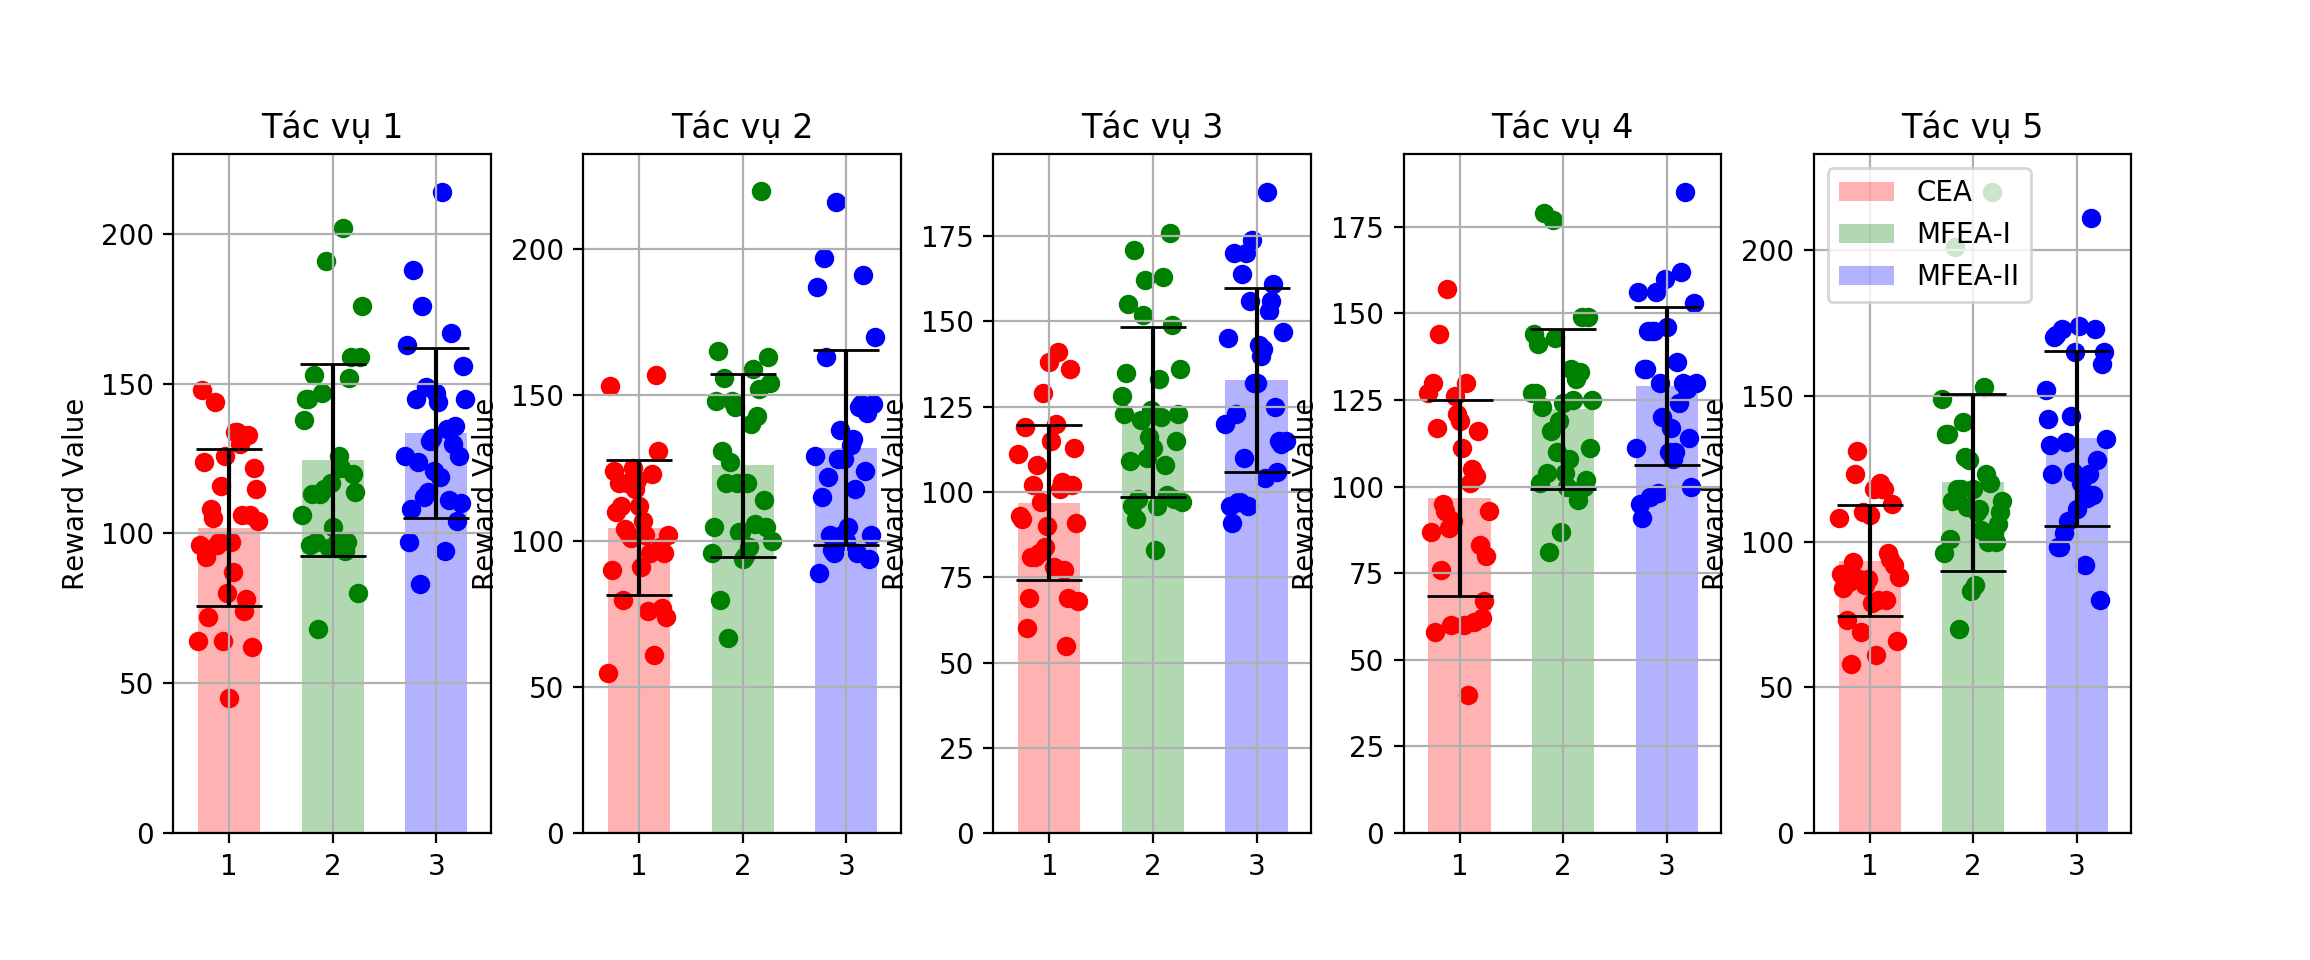
\includegraphics[width=\textwidth,height=\textheight,keepaspectratio]{thesis/images/results/rl/pixelcopter_final.png}
    \caption{Biểu đồ so sánh mức độ tập trung kết quả cuối cùng cho bài toán PixelCopter}
    \label{fig:PixelCopter}
\end{figure}
\subsubsection{Bảng kết quả thực nghiệm - bài toán FlappyBird}
\begin{table} [H]
    \begin{center}
    \caption{Kết quả huấn luyện các tác vụ cho bài toán FlappyBird}

    \scalebox{0.9}{\begin{tabular}{|c|c|c|c|c|c|}
    \hline
    \multirow{1}{*}{\textbf{Thuật toán}} & \multicolumn{1}{c|}{\textbf{Tác vụ 1}} & \multicolumn{1}{c|}{\textbf{Tác vụ 2}} & \multicolumn{1}{c|}{\textbf{Tác vụ 3}} & \multicolumn{1}{c|}{\textbf{Tác vụ 4}} & \multicolumn{1}{c|}{\textbf{Tác vụ 5}} \\ \hline
    CEA & $25.9 \pm 17.57$ & $219.1 \pm 151.39$ & $101.8 \pm 88.65$ & $78.77 \pm 62.43$ & $24.63 \pm 23.62$ \\
    MFEAI & $47.43 \pm 17.97$ & $\mathbf{319.83 \pm 118.9}$ & $\mathbf{217.87 \pm 48.57}$ & $142.9 \pm 26.86$ & $90.17 \pm 20.69$ \\
    MFEAII & $\mathbf{50.93 \pm 16.47}$ & $314.07 \pm 116.25$ & $214.83 \pm 51.96$ & $\mathbf{145.47 \pm 26.72}$ & $\mathbf{105.33 \pm 26.12}$ \\\hline
    \end{tabular}}
    \end{center}
    \label{tab:result:pixelcopter}
\end{table}


\subsubsection{Biểu đồ hội tụ - bài toán FlappyBird}
\begin{figure}[h!]
    \centering
    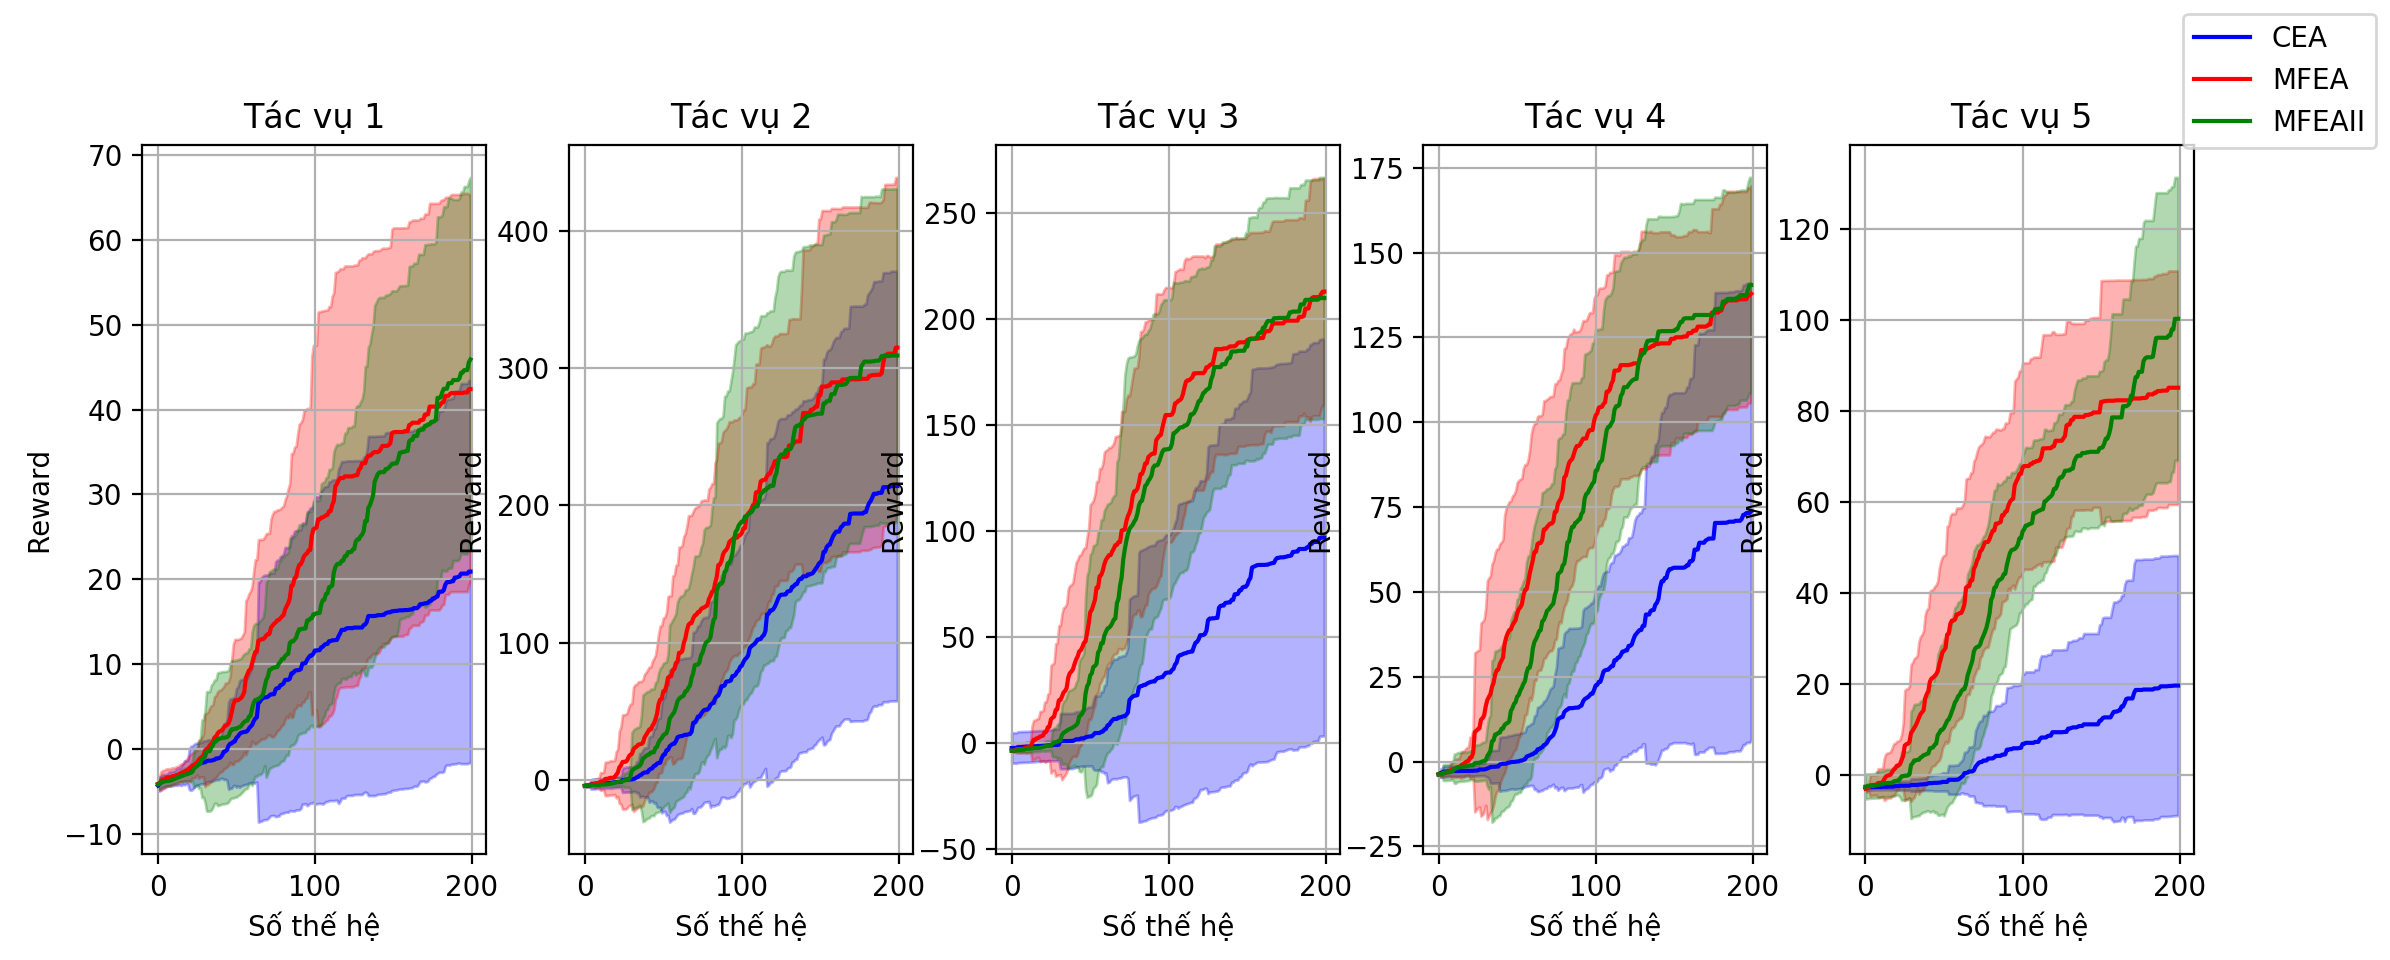
\includegraphics[width=\textwidth,height=\textheight,keepaspectratio]{thesis/images/results/rl/flappybird_conv.png}
    \caption{Biểu đồ hội tụ các tác vụ cho bài toán FlappyBird}
    \label{fig:FLP_conv}
\end{figure}

\subsubsection{So sánh mức độ tập trung kết quả cuối cùng - bài toán FlappyBird}
\begin{figure}[h!]
    \centering
    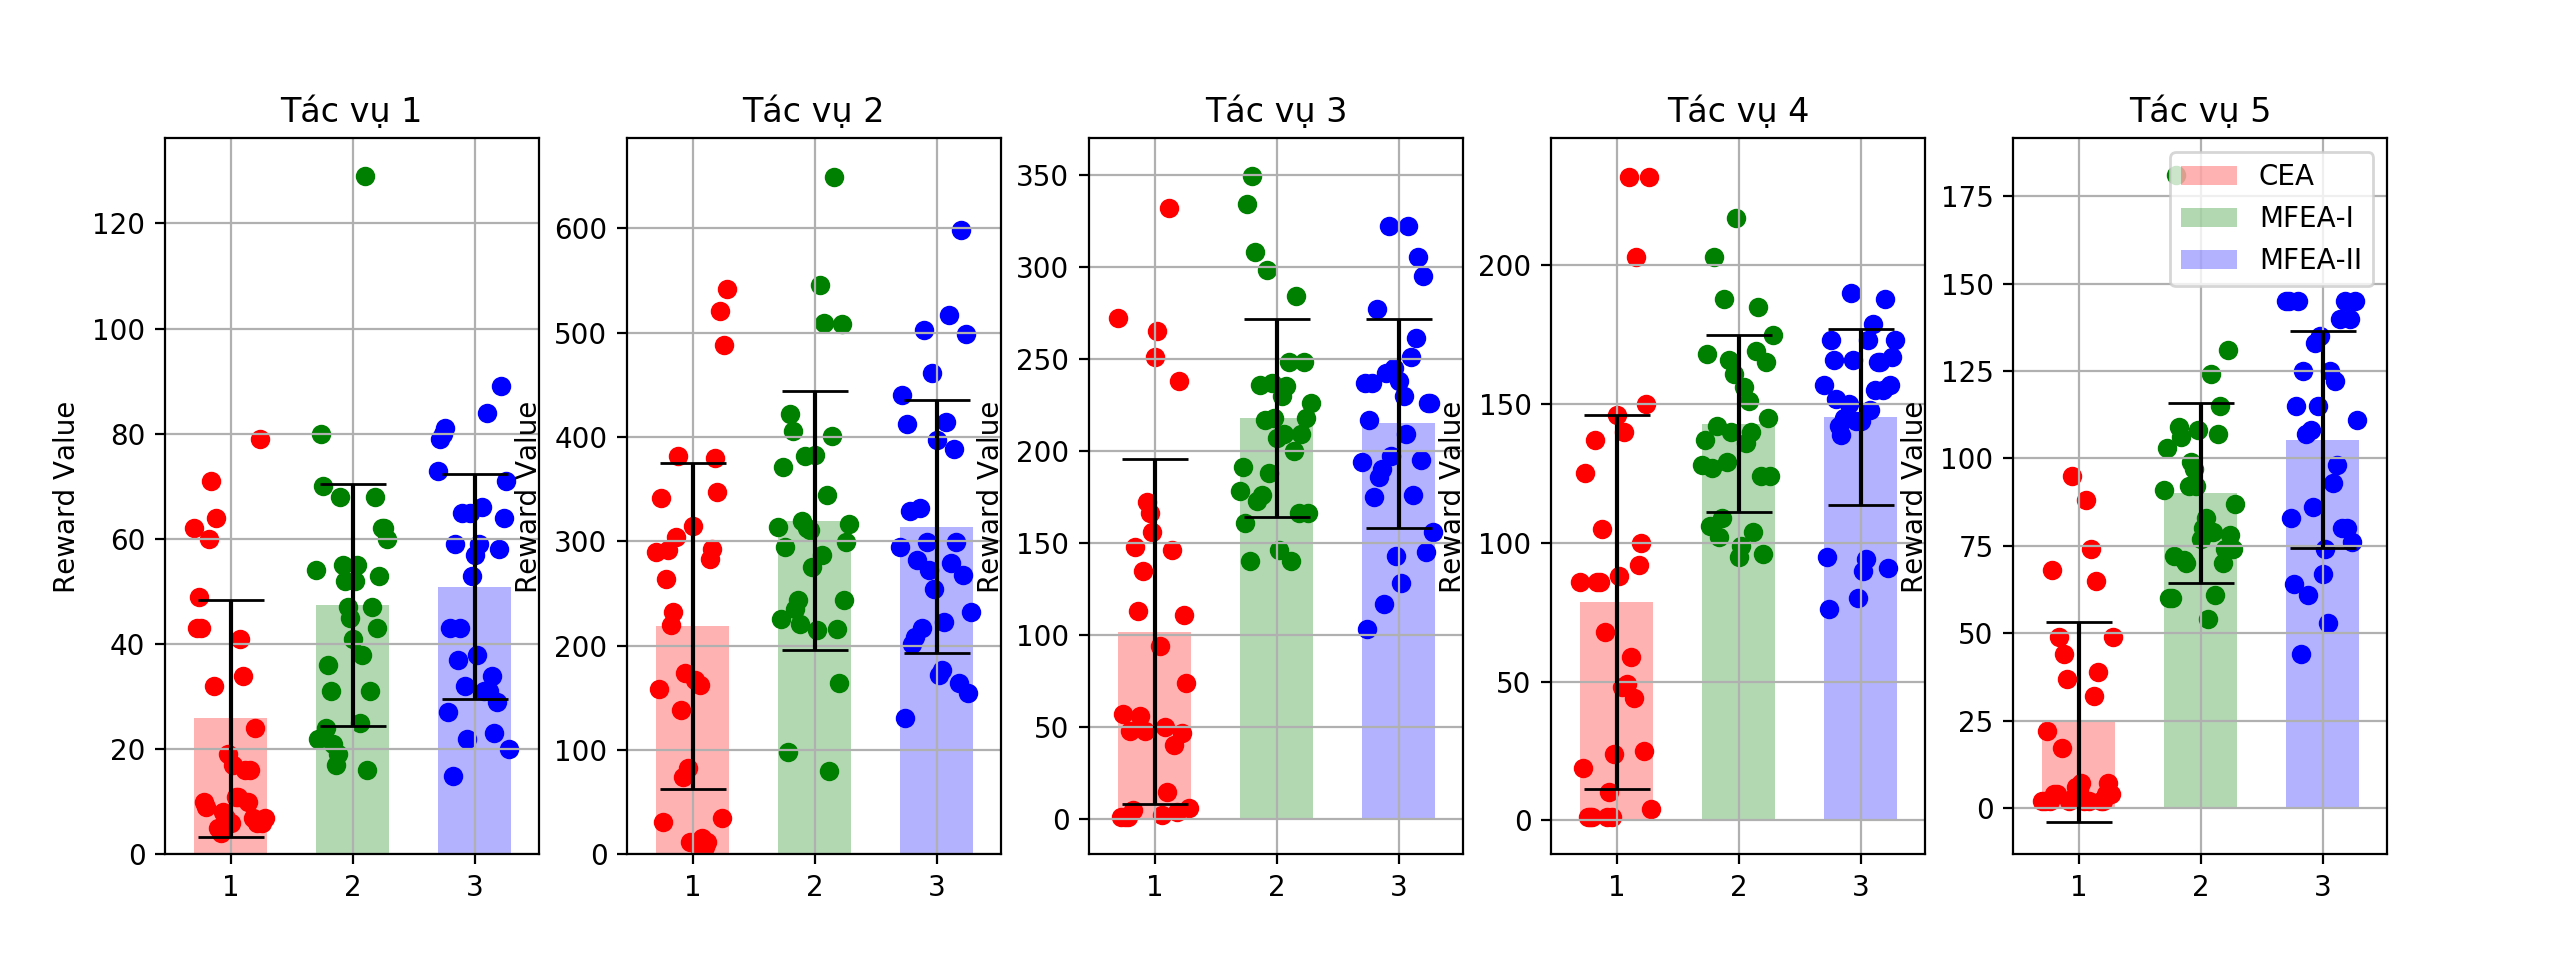
\includegraphics[width=\textwidth,height=\textheight,keepaspectratio]{thesis/images/results/rl/flappybird_final.png}
    \caption{Biểu đồ so sánh mức độ tập trung kết quả cuối cùng cho bài toán FlappyBird}
    \label{fig:FLP}
\end{figure}